\documentclass{article}
\usepackage[utf8]{inputenc}
\usepackage{graphicx}

\title{Tarea 3}
\author{adravel2009 }
\date{September 2020}

\begin{document}

\maketitle

\section{Oscilador armónico simple}

La ecuación diferencial homogénea que se desea resolver y graficar es la siguiente:

\medskip


$\ddot{y} + \omega^2 y=0$

\subsection{Posición vs Tiempo}

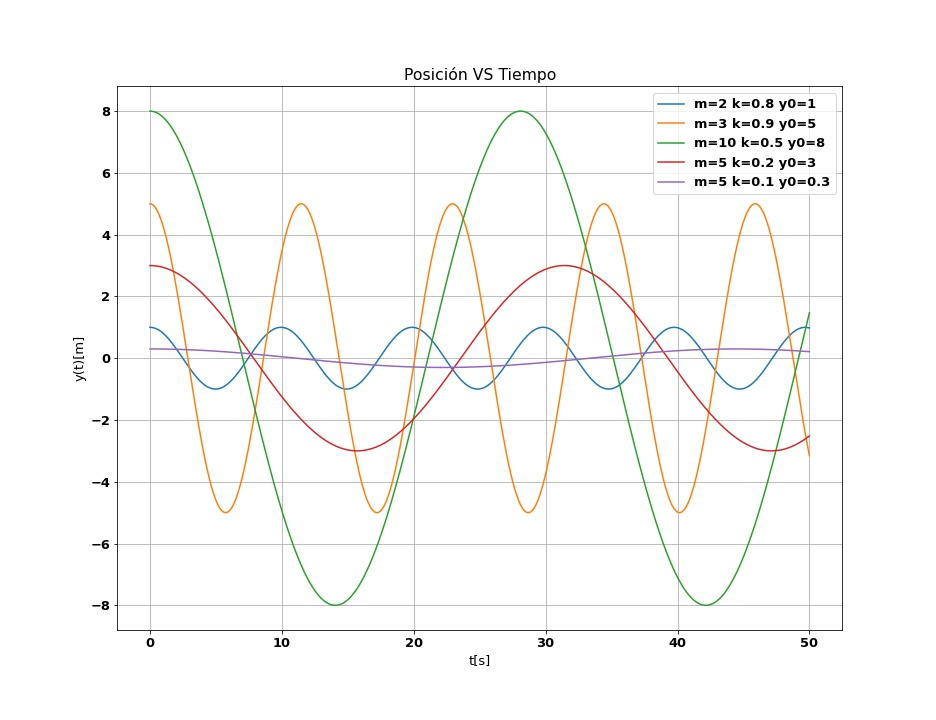
\includegraphics[width=0.7\linewidth]{posición.jpg}

En esta primer gráfica vemos que la solución es cosenoidal y que, como era de esperarse, su amplitud depende de la condición inicial ($y_0$) y para la frecuencia ($\omega$) vemos como entre mayor sea $k$ y menor sea $m$ el movimiento tendrá un frecuencia mayor. Algo a tener en cuenta es que la condición inicial de la velocidad ($v_0$) es igual a cero, es decir, asumimos que el movimiento empieza desde el reposo.

\subsection{Espacio de fase}

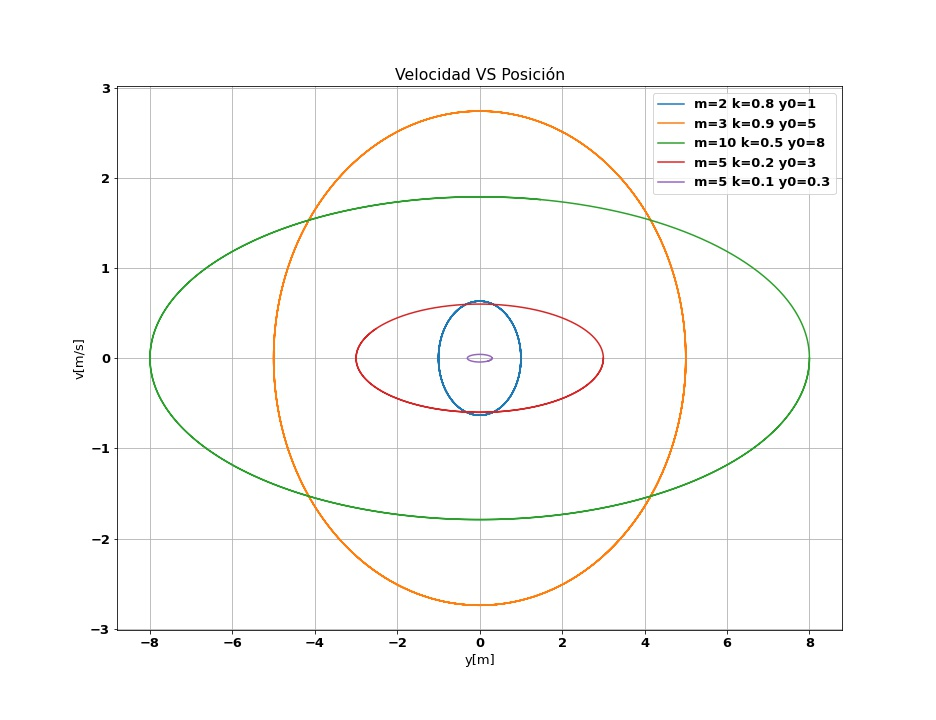
\includegraphics[width=0.7\linewidth]{fases1.jpg}

Vemos una geometría toroidal, lo cual implica que el movimiento es periódico y al hacer el Hamiltoniano del sistema tendremos que no será dependiente del tiempo, trayendo como consecuencia que el Hamiltoniano del sistema es igual a la energía de dicho sistema.


\section{Oscilador armónico subarmortiguado}

\subsection{Posición vs Tiempo}

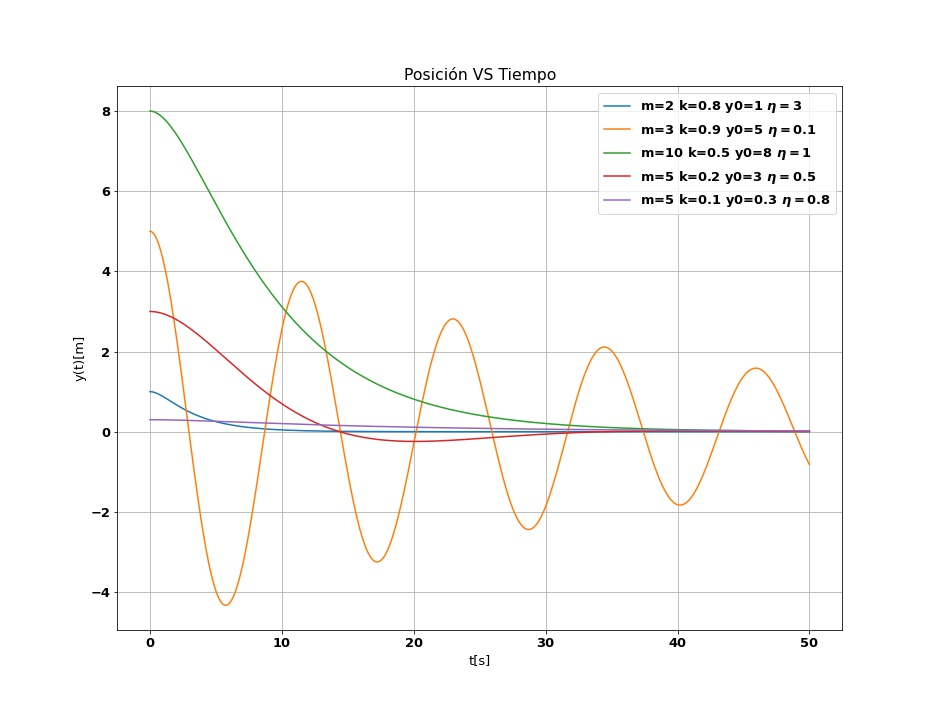
\includegraphics[width=0.7\linewidth]{posición2.jpg}

En está gráfica vemos un decaimiento que depende del valor de $\lambda$, esto nos dice entonces que el sistema está perdiendo energía. La perdida de energía será total hasta dejar a la masa en un estado de reposo.

\subsection{Espacio de fase}

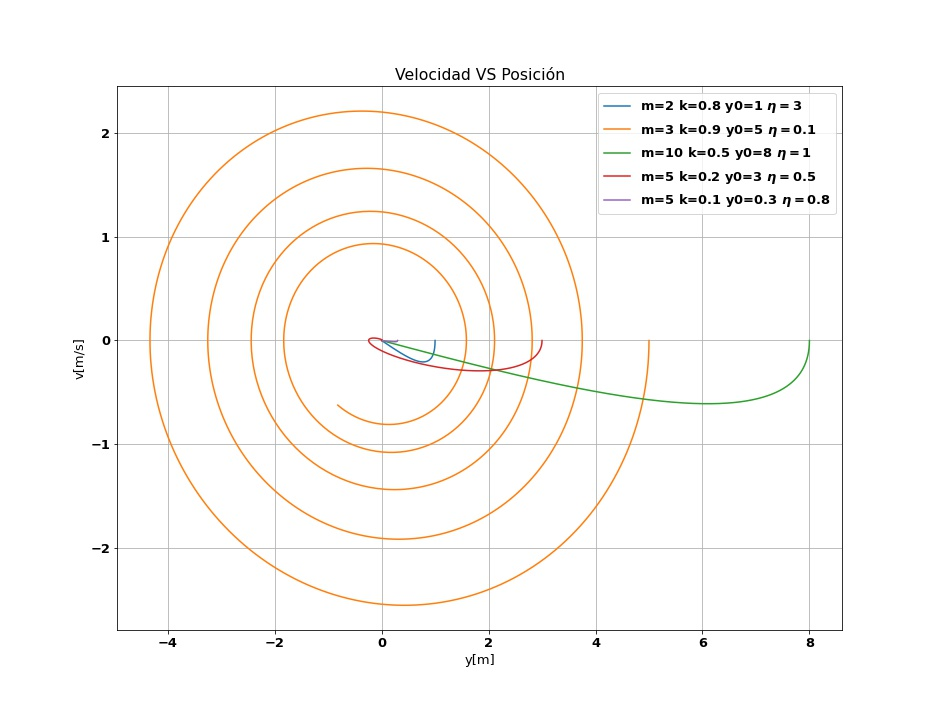
\includegraphics[width=0.7\linewidth]{fases2.jpg}

Para este espacio de fase vemos varios rompimientos de toros, lo cuál implica todo lo contrario que el caso anterior, es decir, el Hamiltoniano dependerá del tiempo haciendo que la energía no se conserve y no es un movimiento periódico.



\end{document}
